\section{Introduction}
With the development of deep learning methods, vision-based vehicle object detection is applied widely in the traffic monitoring area. Unmanned Aerial Systems (UAS) is one of the pioneering monitoring tools of the Intelligent Transportation System infrastructure (ITS)  \cite{Yasin2016ARO}, which measures large areas of traffic network compared to traditional monitoring techniques. However, visual restrictions issues still exist in the UAS monitoring method\ \cite{KIM2023103966}, for example, the vehicles are impeded by trees or shadowed areas. In this situation, existing object detection or tracking methods may lose the vehicle location information.

Seeing through occlusions to obtain a clear background vehicle image without occlusions is a critical task. Due to the varying shape of occlusions, non-fixed location and complexity of reconstructing the details of vehicle images, acquiring occlusion-free vehicle images is still a challenging task. Besides, since the vehicle image obtained from the drone needs to be extracted, there are few mature datasets of vehicle images obtained from the UAS, besides, for studying the vehicle de-occlusion problem, a large scale of occluded vehicle images is required, which is hard to obtain, few types of research exist for solving vehicle de-occlusion problems.

In recent years, thanks to the development of large-scale and high-quality face image datasets, various types of Auto-Encoders (AEs)\ \cite{Zhao2018} or Generative Adversarial Networks (GANs)\ \cite{NIPS2014_5ca3e9b1} could be implemented to solve the face image de-occlusion problem, and significant results are achieved based on such methods.

Inspired by significant achievements in face image de-occlusion areas, we propose an unsupervised visual feature learning algorithm driven by context-based pixel prediction, context encoders\ \cite{Pathak_2016_CVPR}.
Compared to existing image reconstruction methods, this method could reconstruct the image in an unsupervised manner, and it could remove the image by understanding semantic information and by performing representation learning. Moreover, compared to traditional context encoders methods, which could only generate images from a fixed location and occlusion content, this method could generate images with higher flexibility according to the type (tree or shadow) and location of the occlusion mask in a fixed size under the assumption that the location of the mask image is known.

In order to train the updated context encoders, the occluded and non-occluded image pairs are required, therefore, a vehicle dataset with occlusion is needed to build, which corresponds to the ground truth dataset.

The main procedure of this project is based on the updated context encoders network and applying our own training and validating occluded vehicle image dataset, the occlusion-free vehicle images could be generated and the comparison analysis between ground truth and generated images are implemented. The results show that the updated context encoders are able to remove the occlusion and reconstruct the occluded parts and achieve great performance from a qualitative perspective.

This report is organized as follows: in Section 2, we present related works, which inspired us to propose a novel idea. In Section 3, the network structure, loss function and algorithm are introduced to present the pipeline of the proposed work. In Section 4, we introduce the training datasets creation pipeline. In Section 5, the experiment results are analyzed. Finally, conclusions are presented and future work is discussed.


\section{Related work}
Image restoration is the task of transferring a corrupt image into a clean, original image. As shown in \cite{Hosoi2012RestoringOR} and \cite{819578}, PCA can restore occluded images by manipulating the eigenspaces of the training images. However, it has a good performance for the small dataset with specific purposes, like removing sunglasses from the face. A robust-PCA\ \cite{EURECOM+3712} framework is used to detect occlusion masks of input images by a non-occluded facial image set, and generate the occluded parts based on image statistical prior information, while it could obtain a better restoration accuracy, this method could be applied if the occlusion is sparse structure, like grid, stain, text. Sparse coding techniques have been widely used in the field of image restoration\ \cite{2a88c51341cf4974a9d5025abeb86d0d}. However, it is applied to restore the image with corrupted random noise or illumination variation.

Recently, Convolutional Neural Networks (CNNs)\ \cite{Fukushima1980} have greatly improved the performance in unsupervised understanding and generation of natural images. Some of the earliest works in deep unsupervised learning are autoencoders(AEs). AEs are explicitly powerful to remove noise and reconstruct relatively clean images in different scenarios as shown in \cite{Zhao2018, Sagha2017}.
However, because it uses the L2-norm loss function to calculate the similarity between the generated images and corresponding ground-truth images, it often generates blurry images. Similar to Sparse coding techniques, denoising autoencoders reconstruct the image from local corruptions, to make encoding robust to such corruptions. However, those corruptions lack semantic information.

Most closely related to this project are regarding spatial context as a source of the free and abundant supervisory signal. Visual Memex \cite{malisiewicz-nips09} applied context to non-parametrically model object relations and to predict masked objects in scenes, while \cite{Doersch2014} used context to establish correspondences for unsupervised object discovery. However, both approaches relied on hand-designed features and did not perform any representation learning.

Recently, Doersch et al. \cite{vrl} applied the task of predicting the relative positions of neighbouring patches within an image in order to train unsupervised deep feature representations. However, \cite{vrl} are solving a discriminative task rather than a prediction problem.

Image in-painting is the operation of reconstructing missing regions in an image. After GANs have been proposed\ \cite{NIPS2014_5ca3e9b1}, there are an increasing number of works focusing on GANs and their variants for image in-painting tasks. Compared to AEs and their variants, GANs and their variants can acquire sharp details of the images.

Inspired by previous methods, context encoders\ \cite{ce} are introduced, compared to 
\cite{Zhao2018}, \cite{Hosoi2012RestoringOR}, \cite{819578}, context encoders are more robust and generative to the occlusion, compared to
\cite{EURECOM+3712}, \cite{2a88c51341cf4974a9d5025abeb86d0d}, \cite{Sagha2017}, context encoders are able to restore the image with semantic information. Compared to \cite{malisiewicz-nips09}, \cite{Doersch2014}, context encoders are a representation learning method, compared to \cite{NIPS2014_5ca3e9b1}, context encoders are applied to solve a pure prediction problem, it could generate in-painting results by applying an adversary jointly with reconstruction loss and it can be applied to any unlabeled image database and learn to generate images based on the surrounding context. However, the missing area is a binary mask, and the mask region is fixed to the centre region.


Therefore, we present our updated context encoders, which could reconstruct the image with a random mask location and random mask type (tree, shadow), trying to generate the vehicle image without the random mask.


\section{context encoders}
Since the occluded vehicle images are composed of vehicle and occlusion information, which is semantic information, besides, the problem is to reconstruct the occluded part, which is a prediction task, moreover, the occlusion contains several shapes, like a tree, and shadow, and is located in different areas in the vehicle images, therefore, there is a need to apply updated context encoders to solve the occlusion removal problem.

updated context encoders are introduced in this section: it is applying CNN to predict missing parts of a scene based on their surroundings information. An overview of the general architecture is given in Fig. \ref{fig:pipline}, and then details are provided for the learning procedure.
\begin{figure*}[!ht]
	\centering
	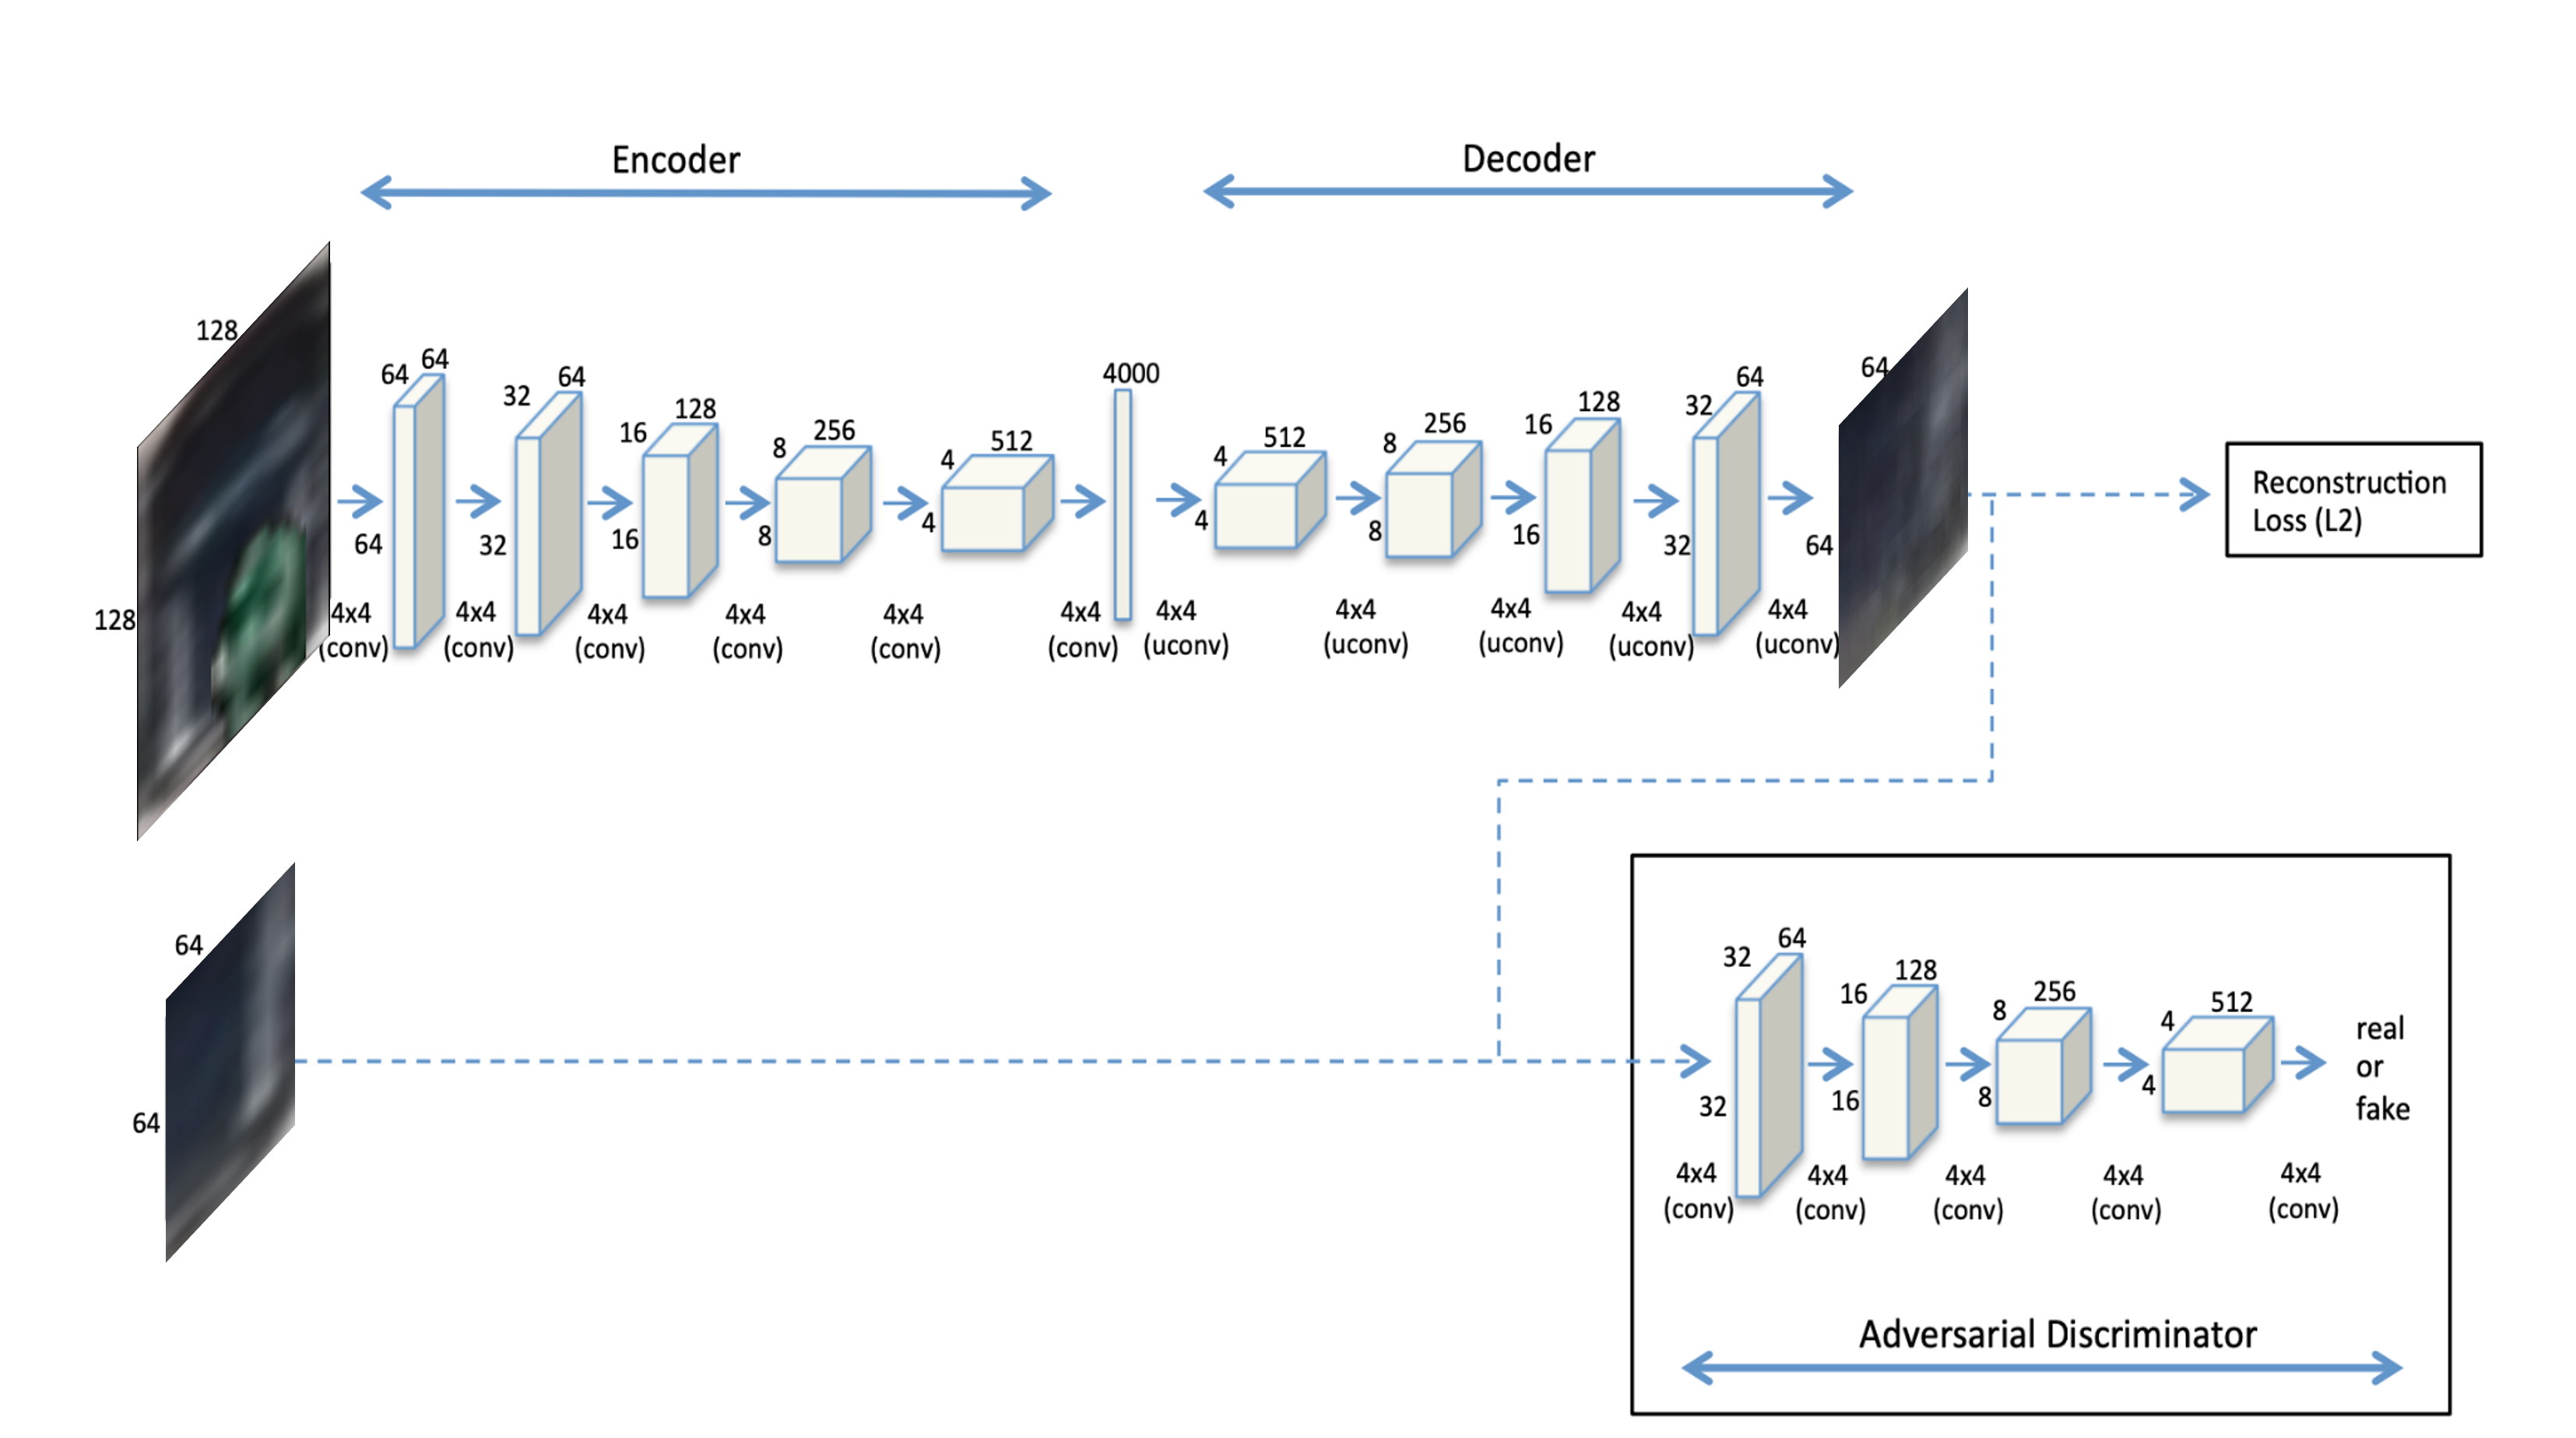
\includegraphics[width=0.9\linewidth]{contents/training pipeline.png}
	\caption{The training pipeline of Context Encoder}
    \label{fig:pipline}
\end{figure*}

\subsection{Encoder-Decoder Pipeline}
The main architecture is a simple encoder-decoder pipeline. The encoder takes an input image with occlusions and outputs a latent feature representation of that image. The decoder takes this latent feature representation and predicts the missing image content. The discriminator is implemented to solve the blurry problem of the prediction.

Since the input size is not unique, and for the convenience of convolution layer size calculation, we resize images to 128 pixels × 128 pixels and then train our joint loss with the resized images. The encoder and discriminator architecture is similar to that of the discriminator in \cite{urldcgan}, and the decoder is similar to the generator in \cite{urldcgan}; the bottleneck is 1 $\times$ 4000 fully connected layer. We applied batch normalization in both the context encoders and discriminator. ReLU \cite{Gonzalez2007} non-linearity is used in the decoder, while leaky ReLU \cite{urldcgan} is implemented in both the encoder and discriminator.

Although this method brings several conveniences for solving the target problem, it also contains several potential limitations. First is the location of the occlusion is required to be an input for training the network. Second, the vehicle or occlusion images should be normalized first, which will occur a non-linear transformation for the image and could change part of the property of the original image. Third, the occlusion image is required to be a fixed-size image, which could be not convenient for solving the real occlusion removal problem.
\subsection{Loss function}
The proposed context encoders are trained by regressing the ground truth content of dropped out the region. However, several equally plausible ways are implemented to replace the missing image region which is consistent with the context. Therefore, this behaviour is modelled by having a decoupled joint loss function to handle both continuities within the context and multiple modes in the output. The reconstruction (\emph{L2}) loss is responsible for capturing the overall structure of the missing region and coherence with regard to its context but prefers to average together the multiple models in predictions. The adversarial loss, on the other hand, tries to let the prediction look real, and has the effect of picking a particular mode from the distribution. For each ground truth image \emph{x}, context encoders \emph{F} produces an output \emph{F(x)}. Let \emph{\^{M}} be an occlusion mask corresponding to the dropped image region with occlusion RGB value matrix. During training, those masks are automatically generated for each image and training loop. We now illustrate the components of the loss function. 

\subsubsection{Reconstruction Loss}
We apply a normalized masked \emph{L2} distance as a reconstruction loss function, $L_{rec}$,

\begin{equation}
    L_{rec}= || \^{M}\textstyle\odot(x-F(1-\^{M}\textstyle\odot x))||^{2}_{2}
\end{equation}
\\
where $\textstyle\odot$  is the element-wise product operation. This simple loss motivates the decoder to produce a rough outline of the predicted object, but it fails to obtain high-frequency detail, which leads to a blurry solution \cite{ce} because in order to minimize the mean pixel-wise loss, it is much easier for \emph{L2} loss to predict the mean of the distribution, which occurs in a blurry averaged image. Therefore, we try to alleviate this issue by adding an adversarial loss.

\subsubsection{Adversarial Loss}

adversarial loss is based on Generative Adversarial Networks (GAN) \cite{NIPS2014_5ca3e9b1}. To learn a generative model \emph{G} of data distribution, GAN tries to learn an adversarial discriminative model \emph{D} to produce loss gradients to the generative model. \emph{G} and \emph{D} are parametric function (e.g., deep networks) where \emph{G} : \emph{Z} $\rightarrow$ \emph{X} maps samples from noise distribution \emph{Z} to data distribution \emph{X}. The learning procedure is a two-player game where an adversarial discriminator \emph{D} acquires both the ground truth and the prediction of \emph{G} and tries to distinguish them, at the same time, \emph{G} tries to confuse \emph{D} by producing samples which are closed to the ground truth as real as possible. The objective for the discriminator is logistic likelihood indicating whether the input is predicted one or the real sample:

\begin{equation}
    \mathop{min}\limits_{G}\mathop{max}\limits_{D} E_{x\in X}[\text{log}(D(x))]+ E_{z \in Z}[\text{log}(1-D(G(z)))]
\end{equation}

This method has recently shown encouraging results in the generative modelling of images. We thus adapt this framework for context prediction by modelling generator by context encoder; i.e., \emph{G}$\triangleq$\emph{F}.  To customize GANs for this task, one could condition the given context information; i.e., the mask $\^{M}\odot x$. However, conditional GANs don’t train easily for context prediction tasks as the adversarial discriminator \emph{D} easily exploits the perceptual discontinuity in generated regions and the original context to easily classify predicted versus real samples. We thus use an alternate formulation, by conditioning only the generator (not the discriminator) on context. The results are improved when the generator was not conditioned on a noise vector. Hence the adversarial loss for context encoders, $L_{adv}$, is:

\begin{equation}
    \mathop{max}\limits_{D}E_{x\in X}[\text{log}(D(x))+\text{log}(1-D(F((1-\^{M})\textstyle\odot x)))]
\end{equation}

where, in practice, both \emph{F} and \emph{D} are optimized jointly using alternating SGD. Note that this objective encourages the entire output of the context encoder to look realistic.
\subsubsection{Joint Loss}
The overall loss function is defined as:
\begin{equation}
    L=\lambda_{rec}L_{rec}+\lambda_{adv}L_{adv}
\end{equation}
\subsection{Region Mask implementation}
\begin{figure*}[!hbt]
    	\centering
    	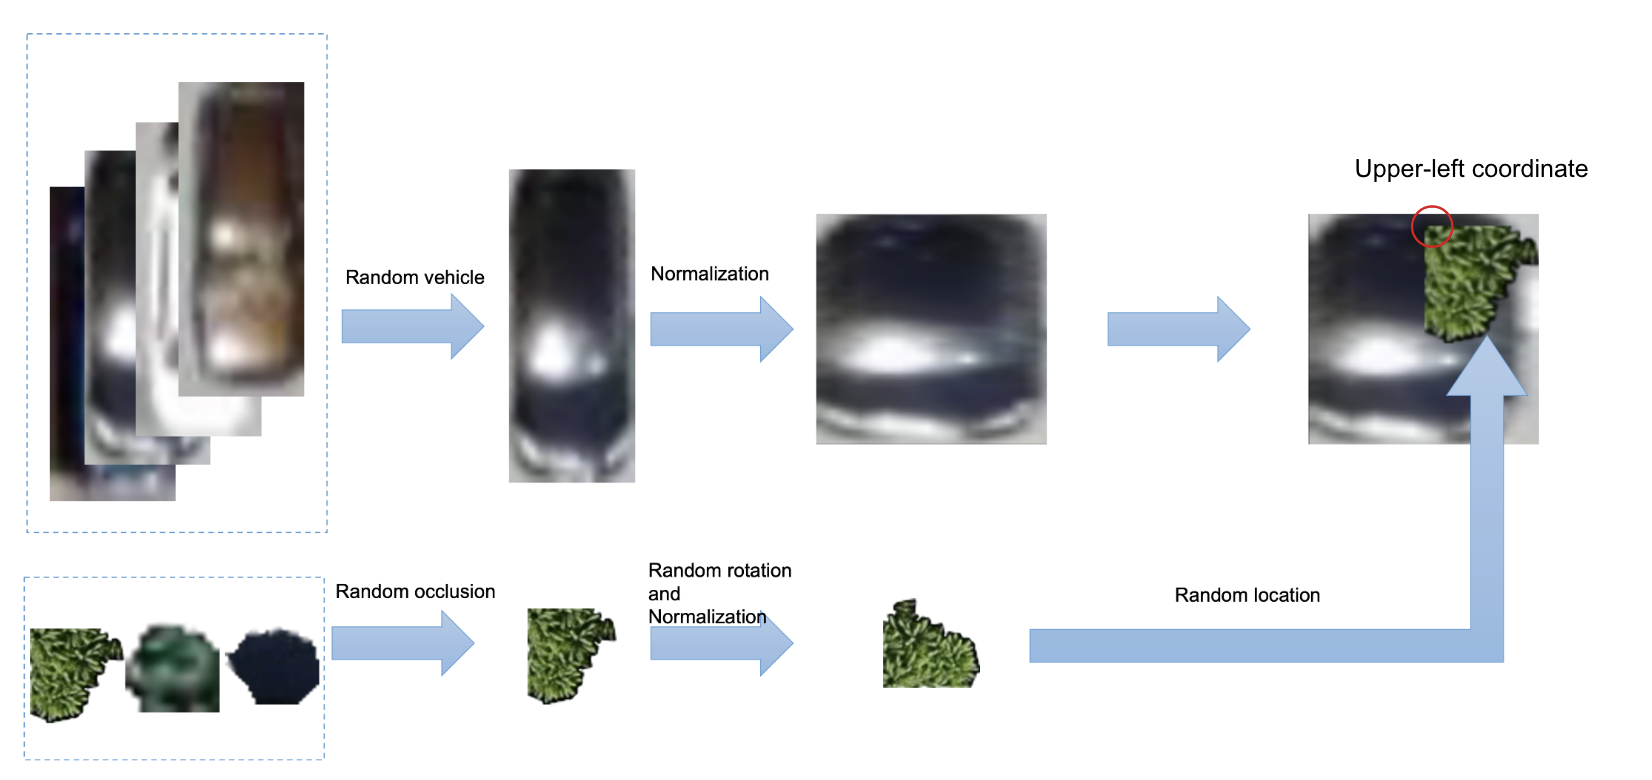
\includegraphics[width=0.9\linewidth]{contents/Dataset creation pipeline.png}
    	\caption{The dataset creation pipeline }
        \label{fig:dataset}
    \end{figure*}
The region mask implementation is similar to the central region mask implementation in \cite{ce}. In the original paper, the mask is a binary mask and the mask location is in the centre of the image. However, in this project, we let the binary mask be a picture, which could be a tree or shadow. Besides, the location is not set in the centre of the image, it could be placed in different locations in the images, which could be found in Fig. \ref{fig:mask}.

\begin{figure}[!ht]
	\centering
	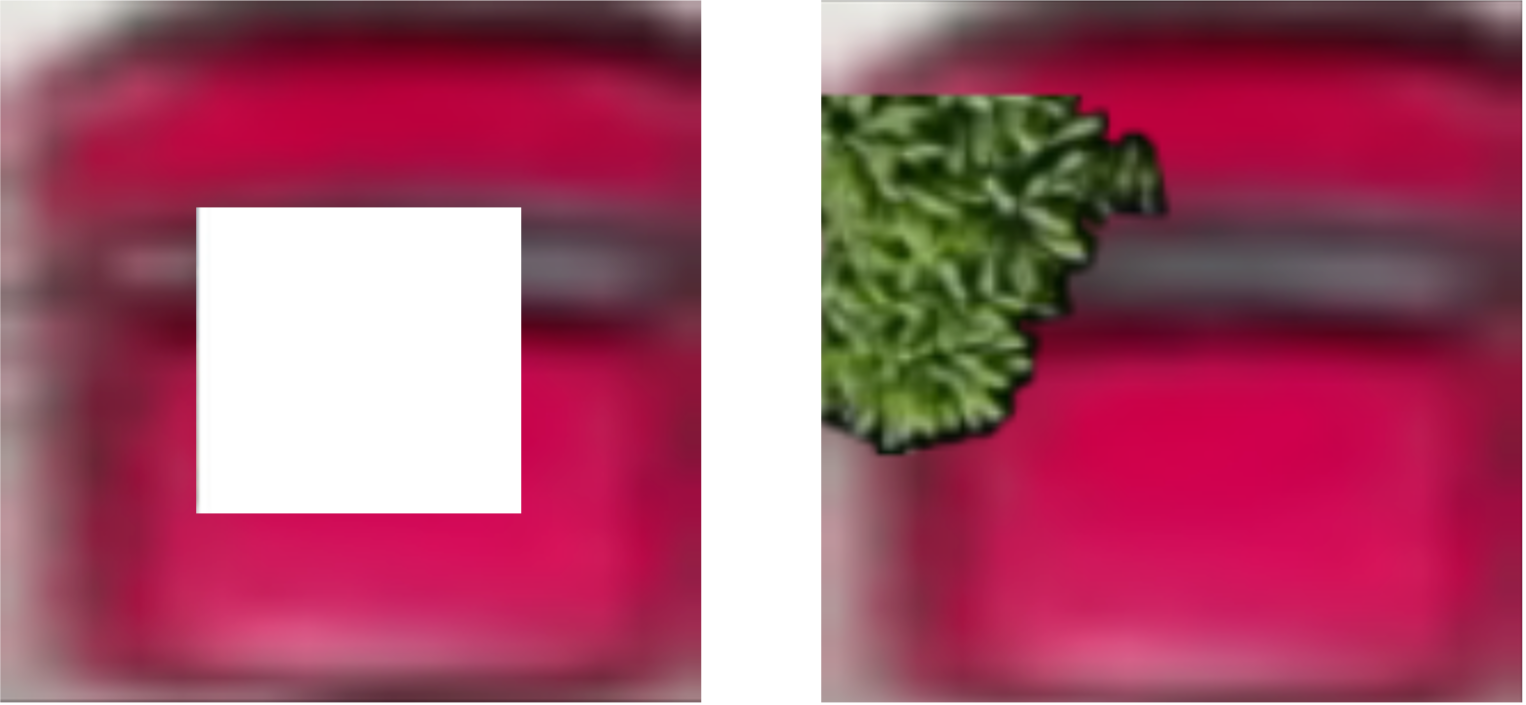
\includegraphics[width=0.9\linewidth]{contents/region comparison.png}
	\caption{The mask comparison of Context Encoder, Left: initial mask, Right: this project's mask.}
    \label{fig:mask}
\end{figure}


\section{Occluded vehicle image dataset creation}

We apply Pully dataset as our own base dataset to train the updated context encoders. Since training the context encoders requires both occluded and occluded-free vehicle image pairs, it is necessary to create our own dataset for training.

In order to build the training dataset, 2 raw datasets are required to build. First is the vehicle dataset, we select 6309 clear vehicle images from the Pully dataset, and put them into the vehicle images folder. Second is the occlusion image dataset, we crop 3 representative images (2 trees and 1 shadow image) from the pully dataset image, and put them into the occlusion image dataset.

The pipeline of creating the training dataset is shown in Fig. \ref{fig:dataset}. The concrete procedure is as follows:
\begin{itemize}
    \item Generate the vehicle image and occlusion randomly from the vehicle images dataset and occlusion images dataset.
    \item Normalize the vehicle image to the size of 128 pixels $\times$ 128 pixels.
    \item Normalize the occlusion image to the size of 64 pixels $\times$ 64 pixels and rotate it at a random angle.
    \item Put the occlusion patch into the vehicle location in a random location and output the occluded vehicle image and the coordinates of the left-upper point of occlusion in the occluded vehicle image.
\end{itemize}
    

\section{Experiment}
\subsection{Dataset}
In this project, 2 datasets are applied. First is the CelebFaces Attributes Datasets (CelebA)\ \cite{7410776}, which contains 202,599 face images, out of this dataset, we select 18041 face images for training. Second is the Pully dataset, which contains 6309 vehicle images. The first dataset is implemented to get the pre-trained weight, and then the pre-trained weight is implemented to train our target dataset.

Besides, we divide our Pully dataset into 2 parts, 80\% samples are applied for the training dataset, and 20\% samples are applied for the validating dataset.
\subsection{Parameters}
In both training procedures, we set the $\lambda_{rec}$ to 0.999 and set the $\lambda_{adv}$ to 0.001, which is suggested in \cite{urldcgan}. For the first training procedure, we apply 80 epochs to train the context encoders and get pre-trained weight. Based on the pre-trained weight, we apply 200 epochs to train the context encoders again.

\subsection{Inferencing}
After finishing the training step, we save the best model weight and input the testing dataset and let the model predict the corresponding results. The procedure is shown in Fig.\ref{fig:inferencing}.
\subsection{Results Analysis}

After the training procedure, we select 12 samples randomly, implement the trained model to predict the result based on the ground truth, and compare the results, which are shown in Fig. \ref{fig:result}.
    \begin{figure}[hbt]
    	\centering
    	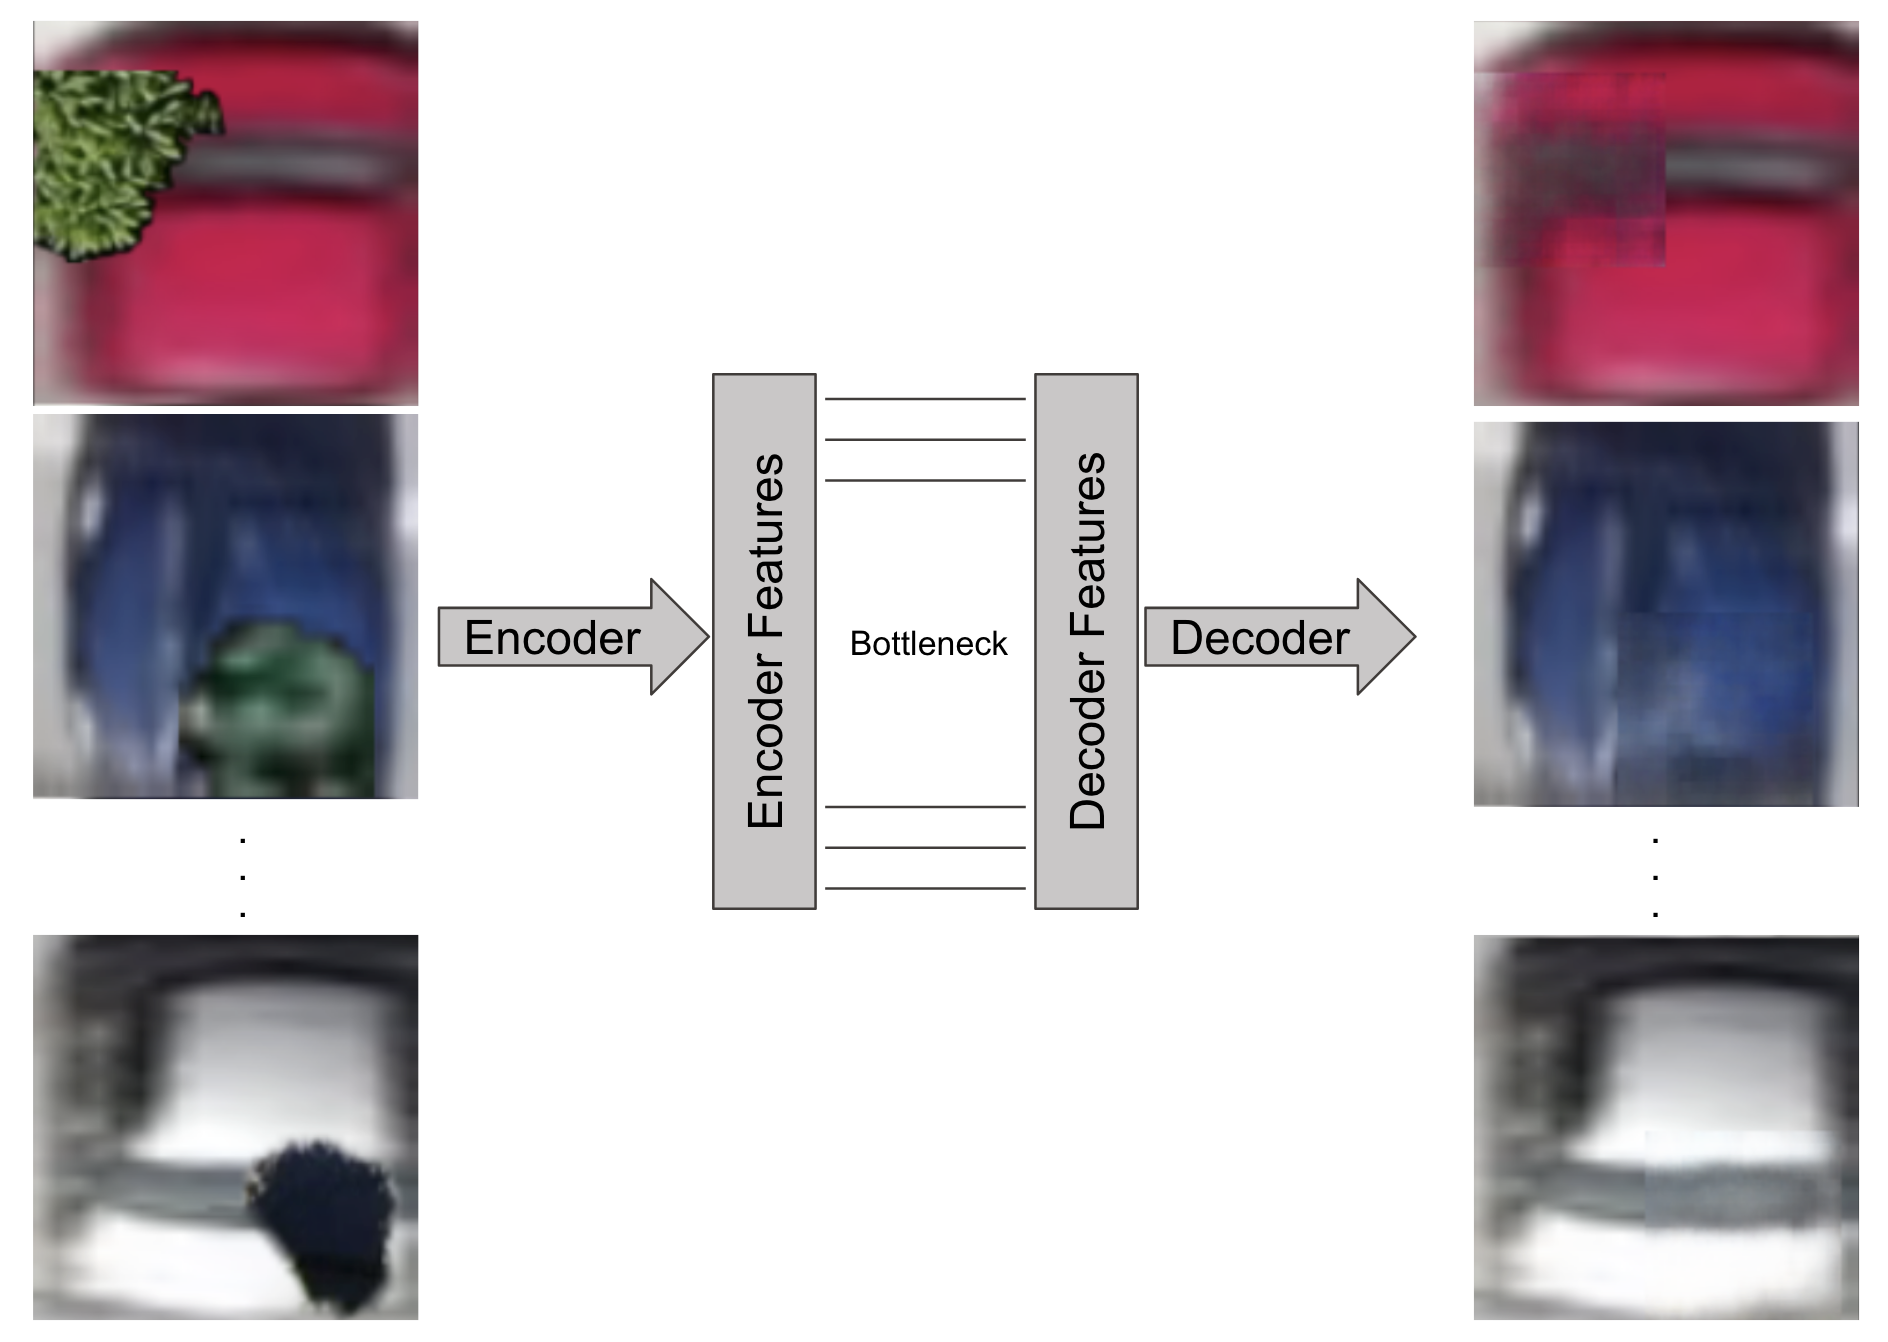
\includegraphics[width=0.9\linewidth]{contents/Inferencing.png}
    	\caption{The inferencing pipeline}
        \label{fig:inferencing}
    \end{figure}
    



From the results, we could see, the main features of the occluded parts are restored successfully, especially if the occluded area contains only one colour, the predicted image and ground truth are hard to tell the difference visually. 

Besides, this method is reliable and stable towards different occlusions. The type of occlusion has a small influence on the generating results.

However, if the occluded parts contain several regions, like the window and the vehicle body. The dividing line between these 2 regions is not so straight, for instance, Fig. \ref{fig:result} (8th subfigure from left),  the  dividing line of the white car between the vehicle's top area and the vehicle window is not so straight.



\section{Conclusion}
In this project, we implemented a new method to remove the occlusion and reconstruct an occlusion-free image semantically by applying the updated context encoders method. For tackling the training dataset missing issue, we apply a dataset creation pipeline to build our own training dataset. Our evaluation shows that our method restores successfully the occluded parts.
\section{Future Work}
Since in this project, we only implement the updated context encoders, the single numerical result is insignificant. In future work, if more methods are implemented, the comparison of the numerical results will be more meaningful.

Although this method brings several conveniences for solving the target problem, it also contains several potential limitations. First, the location of the occlusion is required to be an input for training the network, which is not convenient in real work. Second, the vehicle or occlusion images should be normalized first, which will occur a non-linear transformation for the image and could change part of the property of the original image. Third, the occlusion image is required to be a fixed-size image, which could not be convenient for solving the real occlusion removal problem.
Finally, the vehicle direction is not unique, which means the network needs to learn one more feature from the image, which could affect the performance of the network.

In the future, this project could be improved in the following ways.
\subsection{Two-Stage Occlusion-Aware GAN}

As the \cite{9102788} suggests, the two-stage Occlusion-Aware GAN (OA-GAN) method could be implemented,  which is shown in Fig. \ref{fig:OA-GAN}, where the first GAN is applied for disentangling the occlusions, which will be served as the additional input of the second GAN for synthesizing the final de-occluded faces. Compared to our method, the occlusion location could be detected automatically by this method.
\begin{figure}[!h]
	\centering
	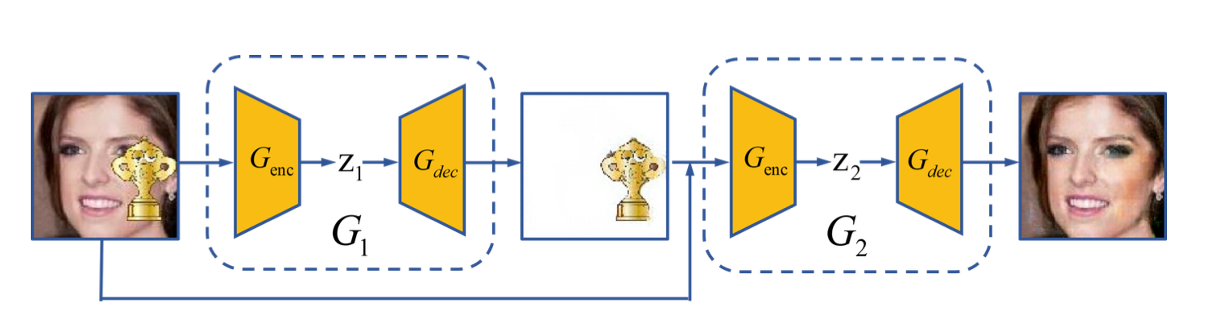
\includegraphics[width=0.9\linewidth]{contents/OA-GAN.png}
	\caption{The structure of two-stage OA-GAN}
    \label{fig:OA-GAN}
\end{figure}

\subsection{Optimized Deep Convolutional Generative Adversarial Networks}

The work of \cite{8608127} proposes an algorithm to infer the mask from an occluded facial image using a novel loss function, and then this mask is applied to in-paint the occlusions automatically by pre-trained DCGANs. As Fig. \ref{fig:DCGAN} displays, it could also detect the mask automatically, and the mask shape could be irregular, which is more flexible than this project's method.
\begin{figure}[!h]
	\centering
	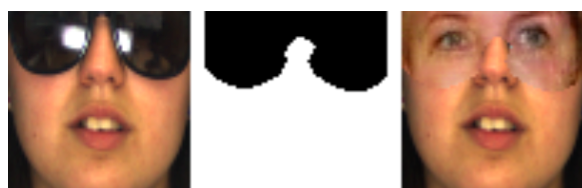
\includegraphics[width=0.9\linewidth]{contents/DCGAN.png}
	\caption{The result of DCGAN. Left: the occluded face image, Middle: learnt mask, Right: final result image.}
    \label{fig:DCGAN}
\end{figure}
\begin{figure*}[!hbt]
	\centering
	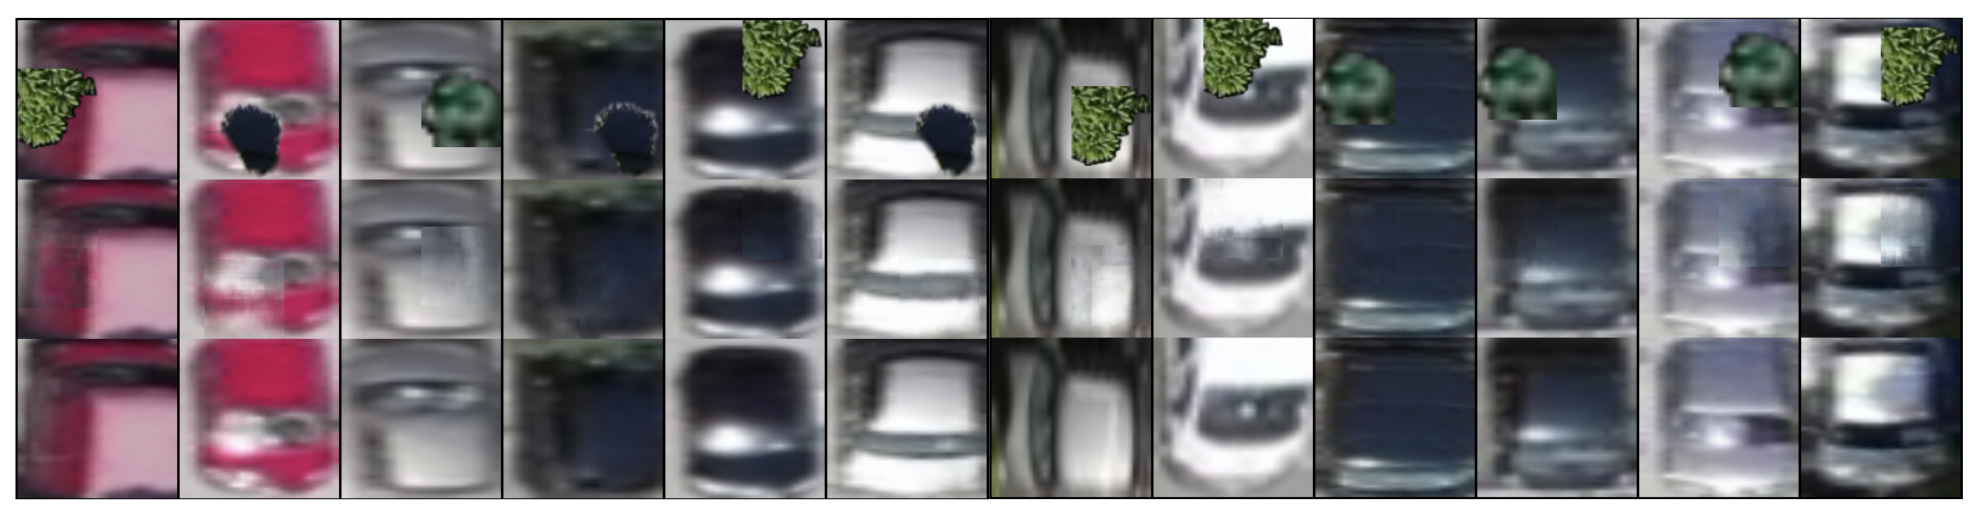
\includegraphics[width=0.9\linewidth]{contents/results.png}
	\caption{The results comparison First row: the vehicle with occlusion, Second row: the predicting results, Third row: the ground truth.}
    \label{fig:result}
\end{figure*}

\subsection{Adding Padding to the Vehicle Image}

Since the input of our method should be fixed-size, we implement the non-linear transformation to normalize every image. However, the non-linear transformation may lose change partial property of the original image. Therefore, we could try to add additional padding to the original image to keep the original image property as well as keep the input size as before, the comparison is shown in Fig. \ref{fig:padding}.
\begin{figure}[!ht]
	\centering
	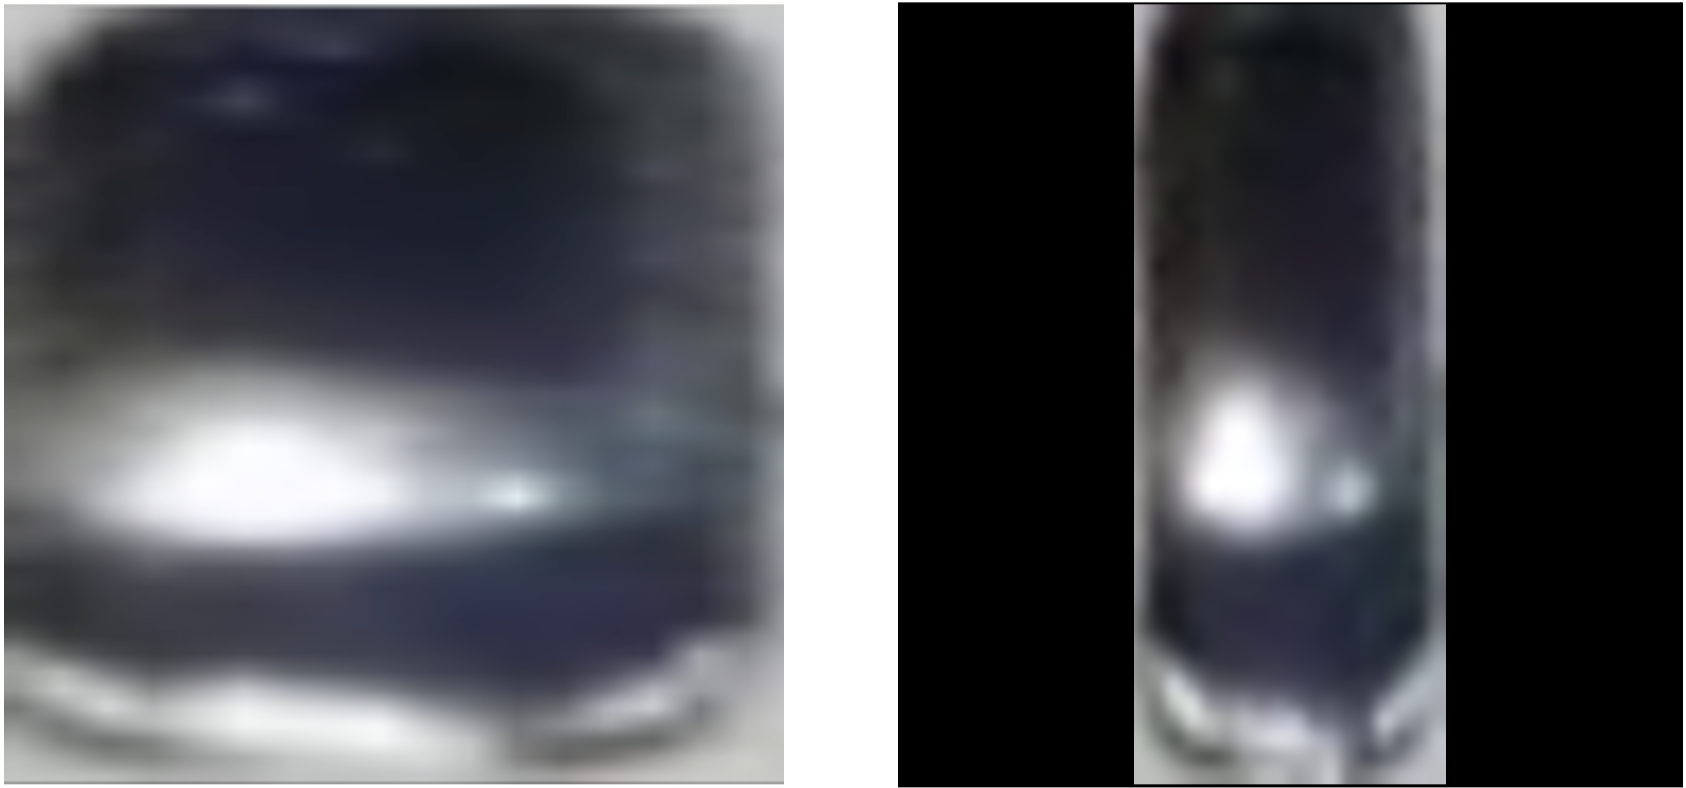
\includegraphics[width=0.7\linewidth]{contents/padding and stretching.png}
	\caption{The comparison between non-linear transformation and padding adding method. Left: non-linear transformation. Right: padding adding method.}
    \label{fig:padding}
\end{figure}
\subsection{Direction Normalization Method}

From Fig. \ref{fig:result}, it could be seen that the direction of the vehicle is not unique, which may cause the network to learn one more feature so that the reconstruction effect may be reduced. Therefore, the direction normalization method could be implemented before training the model, as shown in Fig. \ref{fig:DNM}.
    
\begin{figure}[!ht]
	\centering
	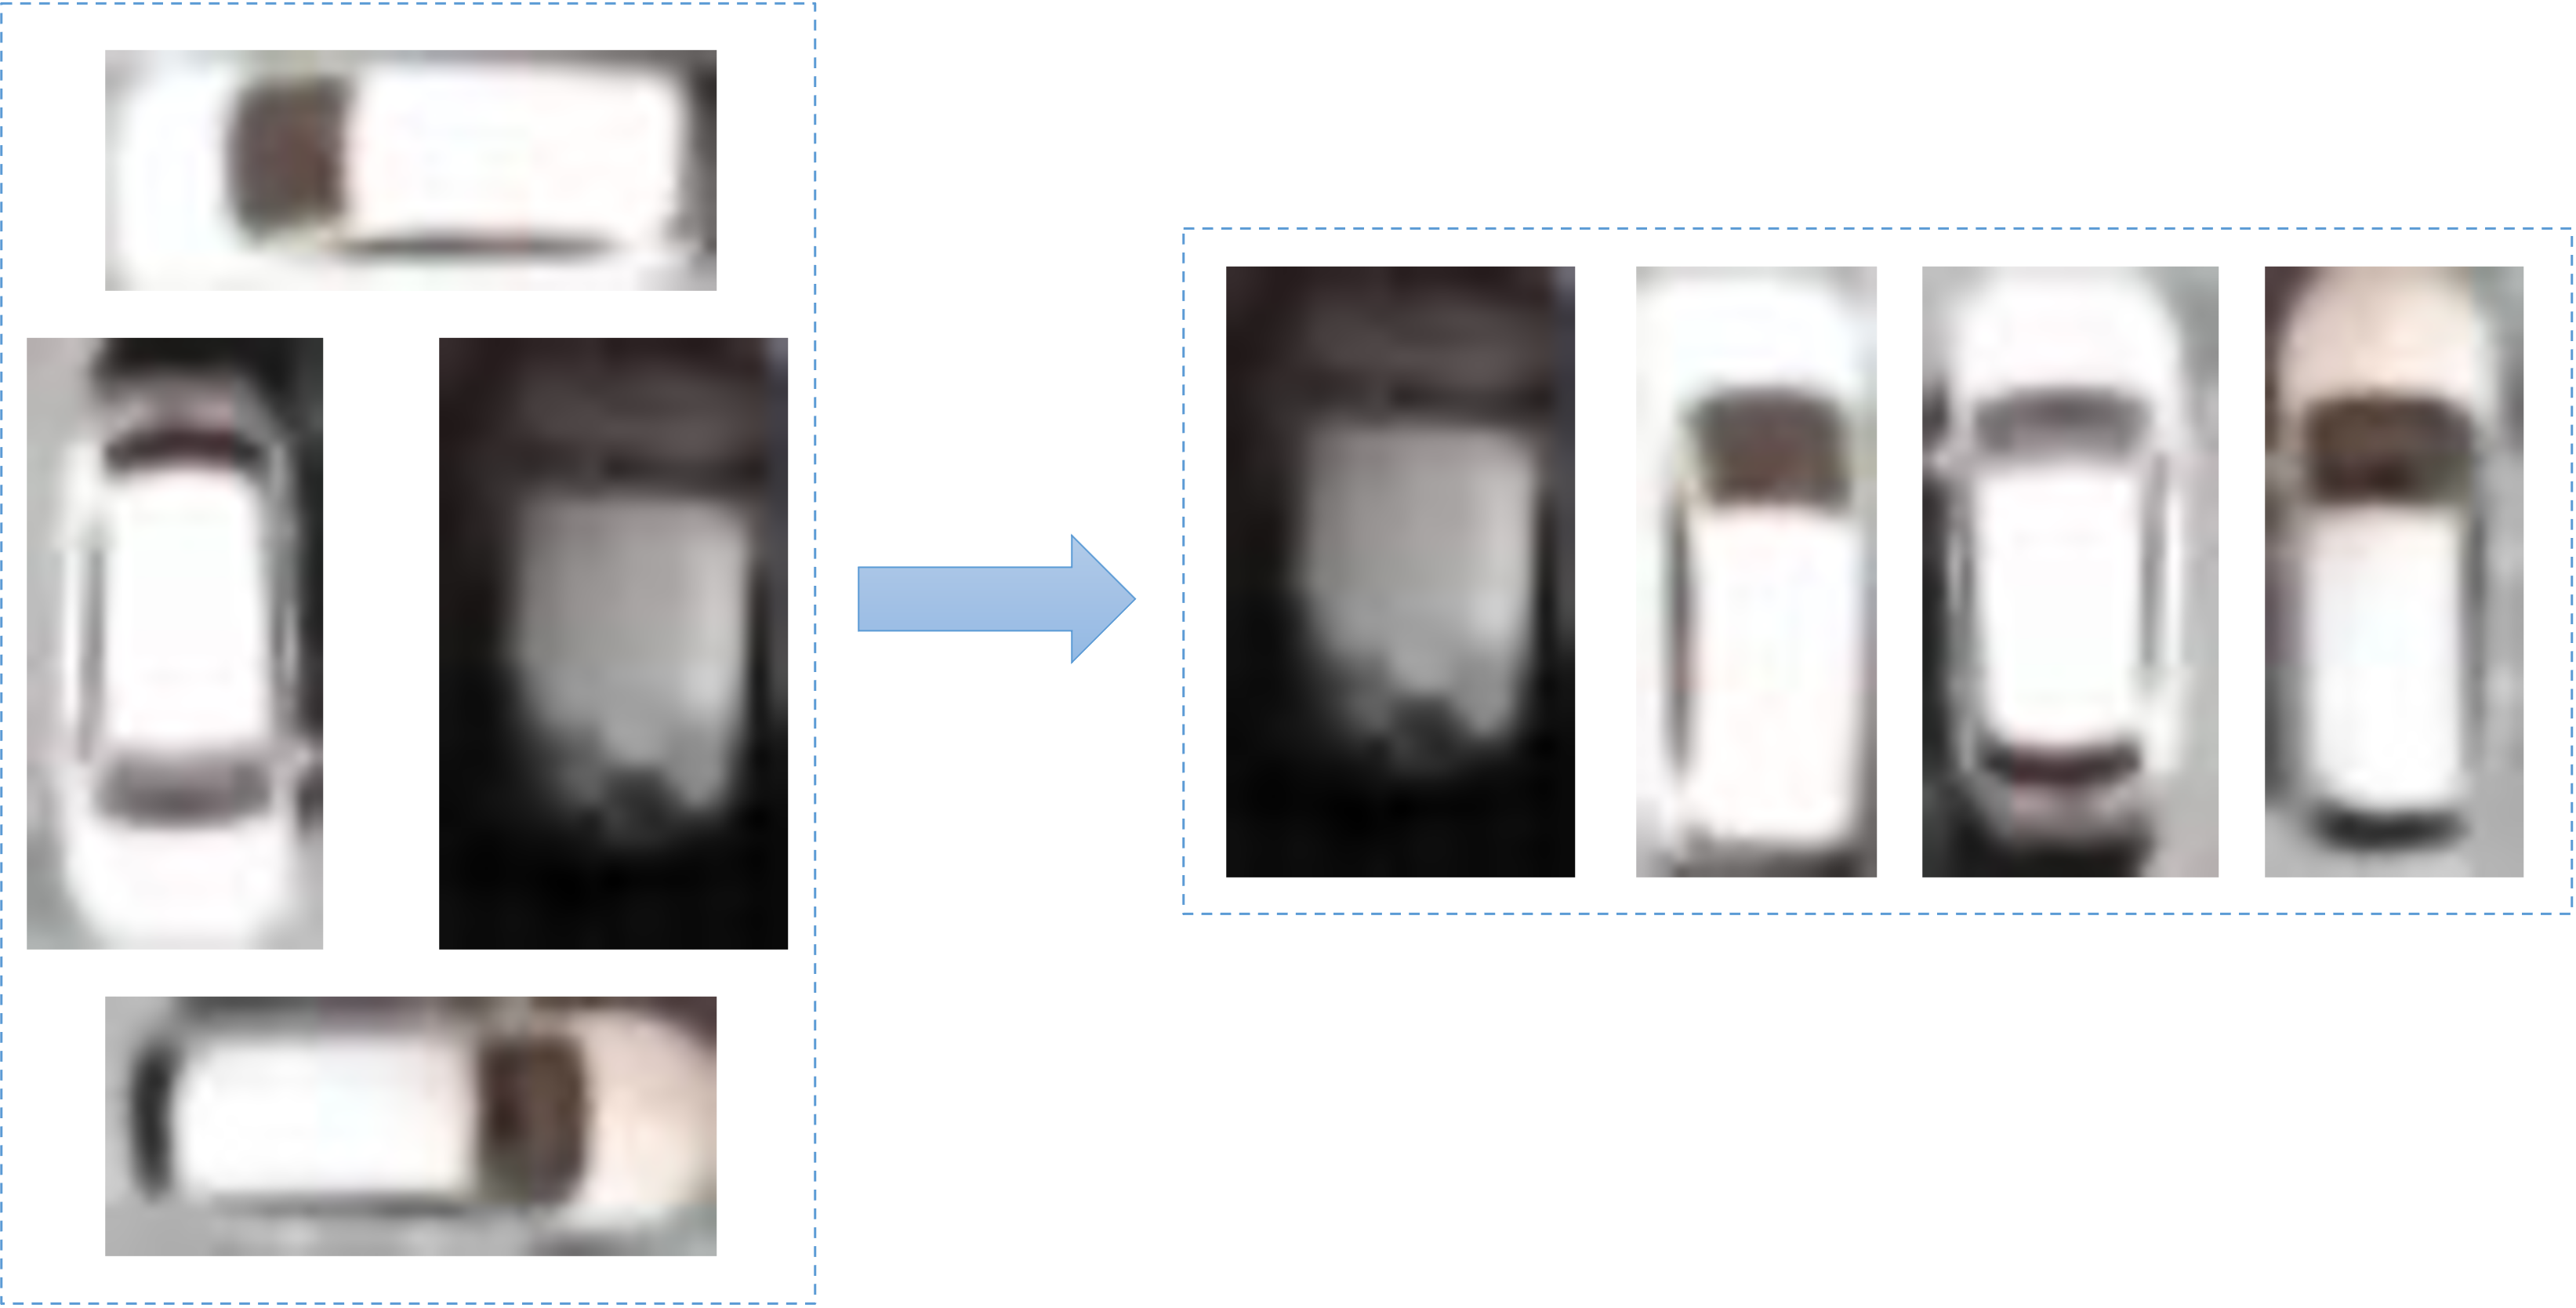
\includegraphics[width=0.9\linewidth]{contents/direction normalization method.png}
	\caption{Direction normalization method. Left: the original images. Right: the images after direction normalization.}
    \label{fig:DNM}
\end{figure}


